\documentclass[11pt,a4paper]{article}

\usepackage[utf8]{inputenc}
\usepackage[T1]{fontenc}
\usepackage[spanish,es-tabla]{babel}
\usepackage[margin=2.35cm]{geometry}
\usepackage{amsmath}
\usepackage{amssymb}
\usepackage{graphicx}
\usepackage{booktabs}
\usepackage{array}
\usepackage{float}
\usepackage{xcolor}
\usepackage{colortbl}
\definecolor{bestrow}{RGB}{220,245,220}
\definecolor{altrow}{RGB}{235,243,255}
\definecolor{worstrow}{RGB}{255,230,230}
\usepackage{microtype}
\usepackage{hyperref}
\usepackage{listings}
\usepackage{enumitem}
\usepackage{caption}

\microtypesetup{expansion=false}

\hypersetup{
    colorlinks=true,
    linkcolor=blue!60!black,
    citecolor=blue!60!black,
    urlcolor=blue!60!black
}

\lstdefinestyle{codestyle}{
    basicstyle=\ttfamily\small,
    breaklines=true,
    frame=single,
    columns=fullflexible,
    keepspaces=true,
    showstringspaces=false,
    tabsize=2,
    backgroundcolor=\color{gray!5}
}

\lstset{style=codestyle}

\graphicspath{{artifacts/figures/}}

\setlist[itemize]{leftmargin=1.2em}
\setlist[enumerate]{leftmargin=1.4em}

\title{\textbf{Predicción de fallos APS en camiones Scania}\\
\large Mantenimiento predictivo con datos tabulares, coste asimétrico, explicabilidad y robustez}

\author{
    Mauro Valls Vidal\\
    Alejandro Parra Sánchez\\
    Jordi Blasco Lozano\\
    Alejandro Martínez Riquelme\\[0.4em]
    \small Grado en Ingeniería en Inteligencia Artificial\\
    \small Escuela Politécnica Superior, Universidad de Alicante\\
    \small Aprendizaje Avanzado
}

\date{Curso 2025--2026}

\begin{document}

\maketitle

\begin{abstract}
Este trabajo presenta un estudio de aprendizaje automático para detectar fallos relacionados con el sistema APS de camiones Scania. La tarea se formula como clasificación binaria sobre datos tabulares industriales con 170 variables predictoras, valores faltantes, variables anonimizadas y una clase positiva muy minoritaria. El objetivo es identificar fallos APS y reducir el riesgo de falsos negativos. Los modelos se comparan mediante \texttt{Pipeline}, \texttt{GridSearchCV} y validación cruzada estratificada de 5 folds usando únicamente train. El mejor estimador se reentrena con todo train mediante \texttt{refit} y test queda reservado para la evaluación final. Se comparan un baseline, modelos lineales, SVM lineal, árboles y ensembles. El modelo principal seleccionado es \texttt{HistGradientBoosting}, con PR-AUC media de 0.881 en validación cruzada. En test obtiene PR-AUC de 0.922, F1 positivo de 0.842, recall positivo de 0.752, 13 falsos positivos y 93 falsos negativos. La memoria añade análisis de coste asimétrico, anomalías, importancia por permutación, robustez, errores y shift. La conclusión es que \texttt{HistGradientBoosting} es el modelo principal defendible, mientras que \texttt{logistic\_class\_weight} queda como alternativa operativa si se prioriza coste.
\end{abstract}

\noindent\textbf{Palabras clave}
Mantenimiento predictivo, Scania APS, clasificación binaria, datos tabulares, desbalanceo, PR-AUC, coste asimétrico, explicabilidad, robustez.

\tableofcontents
\newpage

\section{Introducción}
\label{sec_intro}

El mantenimiento predictivo busca anticipar fallos antes de que se conviertan en averías costosas. En vehículos industriales, una detección temprana puede reducir paradas, reparaciones innecesarias y riesgos operativos. Este proyecto se centra en el sistema APS de camiones Scania, relacionado con el suministro de aire a presión. Un fallo de este sistema puede afectar al funcionamiento del vehículo y generar costes importantes.

El problema tiene una dificultad práctica clara. Los fallos APS reales son poco frecuentes, por lo que la clase positiva aparece muy poco frente a la clase negativa. En este contexto, un modelo puede obtener una accuracy alta aunque ignore casi todos los fallos reales. Por esta razón, el proyecto no se evalúa solo con accuracy. Se usan métricas centradas en la clase positiva como recall, F1 y PR-AUC, junto con un coste asimétrico que penaliza más los falsos negativos.

La motivación del aprendizaje automático es aprovechar señales presentes en sensores, contadores y agregados internos del camión. Aunque las variables están anonimizadas, sus patrones estadísticos pueden ayudar a distinguir casos APS de casos no APS. La anonimización limita la interpretación física directa, pero no impide construir un modelo predictivo si el protocolo experimental se diseña con cuidado.

El objetivo del trabajo es construir y evaluar un flujo reproducible de aprendizaje automático para detectar fallos APS. El sistema no se presenta como una solución de producción. Es un estudio académico y técnico que compara modelos, analiza errores y discute limitaciones.

Las contribuciones del trabajo se resumen en cuatro puntos. Primero, se construye un flujo reproducible de preparación, exploración, modelado y auditoría para el dataset APS. Segundo, se comparan modelos de familias distintas bajo un protocolo común con \texttt{Pipeline}, \texttt{GridSearchCV} y validación cruzada de 5 folds. Tercero, se incorpora una lectura operativa del problema mediante coste asimétrico, análisis de falsos negativos y comparación de estrategias sensibles al desbalanceo. Cuarto, se añaden análisis complementarios de anomalías, explicabilidad, robustez y shift que permiten interpretar el comportamiento del modelo más allá de una única métrica final.


\section{Contexto y trabajo relacionado}
\label{sec_contexto}

\subsection{Mantenimiento predictivo}

El mantenimiento predictivo consiste en usar datos históricos del sistema para estimar si puede aparecer un fallo antes de que ocurra una avería grave. La idea no es esperar a que el camión falle, como ocurre en el mantenimiento correctivo, ni revisar siempre cada cierto tiempo aunque no haya indicios de problema, como ocurre en el mantenimiento preventivo tradicional.

En este enfoque, las revisiones se intentan adaptar al estado real del vehículo. Si los datos de los sensores indican un comportamiento anómalo, el sistema puede recomendar una revisión antes de que el fallo cause una parada o una reparación más costosa.

En camiones y otros vehículos industriales, esto es especialmente útil porque una avería puede dejar el vehículo inmovilizado, generar retrasos y aumentar los costes de mantenimiento. Sin embargo, el modelo debe evaluarse con cuidado. Un falso positivo implica revisar un camión que realmente no tenía fallo APS. Un falso negativo implica no detectar un fallo real. En este proyecto, el falso negativo es el error más grave porque puede dejar pasar una avería que debería haberse anticipado.

\subsection{Clasificación tabular y desbalanceo}

El dataset APS es tabular. Cada fila representa un caso de mantenimiento y cada columna describe una señal numérica. Este tipo de problema suele beneficiarse de árboles, bosques aleatorios y métodos de boosting, aunque los modelos lineales siguen siendo útiles como referencia.

El desbalanceo es una característica central del problema. Como hay muy pocos casos positivos, un modelo podría acertar muchos negativos y aun así fallar justo en los fallos APS que interesa detectar. Por eso la accuracy puede dar una impresión demasiado optimista. En su lugar se usan métricas centradas en la clase positiva, como recall, F1 y PR-AUC. PR-AUC es especialmente útil porque evalúa cómo de bien el modelo prioriza los casos positivos cuando estos son escasos.

\subsection{Coste, explicabilidad y robustez}

En un problema industrial no todos los errores pesan igual. El dataset define un coste de 10 para falsos positivos y de 500 para falsos negativos. Este esquema no captura toda la complejidad real del mantenimiento, pero permite estudiar el impacto operativo de los errores.


La explicabilidad también importa. En este proyecto se usa importancia por permutación, que consiste en desordenar una variable y medir cuánto empeora el modelo, para estimar qué variables influyen más en sus predicciones. Esta técnica no demuestra causalidad. Sirve para auditar dependencias del modelo y detectar si el rendimiento depende de pocas variables.

La robustez se analiza añadiendo ruido a variables numéricas. Esta prueba no equivale a una validación de producción, pero ayuda a observar si pequeñas perturbaciones degradan mucho el rendimiento. Gracias a este análisis se puede valorar si el modelo sería sensible a errores, ruido o pequeñas variaciones en las mediciones de los sensores.

\section{Descripción del problema y los datos}
\label{sec_problema_datos}

\subsection{Definición del problema}
\label{sec_definicion_problema}

El sistema propuesto está pensado como una herramienta de apoyo para equipos de mantenimiento, responsables de flota o personal técnico que necesite priorizar revisiones de camiones. La salida del modelo no debe interpretarse como una decisión automática de reparación. Su función sería señalar casos con riesgo de fallo APS para que una persona experta pueda revisarlos con más información.

La tarea se define como clasificación binaria. Cada observación \(x_i\) contiene 170 variables numéricas procedentes del sistema del camión. La etiqueta \(y_i\) toma valor 0 si el caso no está relacionado con APS y valor 1 si el fallo sí está relacionado con APS.

\[
f(x_i) \rightarrow \hat{y}_i \in \{0,1\}
\]

Las consecuencias de los errores no son simétricas. Un falso positivo implica revisar un camión que finalmente no presenta fallo APS. Esto puede aumentar el coste de inspección y generar trabajo adicional. Un falso negativo implica no detectar un fallo APS real. Este error es más delicado porque puede retrasar una intervención necesaria y aumentar el coste operativo posterior. Por ello, el proyecto presta especial atención al recall de la clase positiva, al coste y al análisis de falsos negativos.

\subsection{Origen y características del dataset}
\label{sec_dataset}

El dataset usado es \textit{APS Failure at Scania Trucks} del UCI Machine Learning Repository. Es un dataset tabular suficientemente rico para el objetivo del proyecto, ya que contiene decenas de miles de instancias y 170 variables predictoras. Proporciona una partición oficial de entrenamiento y otra de test. La Tabla \ref{tab_dataset} resume sus características principales.

\begin{table}[H]
\centering
\caption{Características principales del dataset}
\label{tab_dataset}
\small
\begin{tabular}{@{}lr@{}}
\toprule
\textbf{Elemento} & \textbf{Valor}\\
\midrule
Train & 60000 filas\\
Test & 16000 filas\\
Variables predictoras & 170\\
Tipo de datos & Tabulares numéricos\\
Clase negativa original & \texttt{neg}\\
Clase positiva original & \texttt{pos}\\
Codificación usada & \texttt{neg} como 0 y \texttt{pos} como 1\\
Coste de falso positivo & 10\\
Coste de falso negativo & 500\\
\bottomrule
\end{tabular}
\end{table}

Las variables predictoras están anonimizadas. Proceden de sensores, contadores o agregados internos del camión, pero no se conoce su significado físico exacto. Esta anonimización es una limitación importante, porque dificulta interpretar por qué una variable concreta está asociada al fallo. Por ello, la memoria distingue entre importancia estadística e interpretación causal.

Los valores faltantes aparecen marcados como \texttt{na} en los archivos originales. Esos valores no son valores faltantes reales al cargarlos directamente, sino texto que indica ausencia de dato. Por eso, durante la preparación se convierten a valores faltantes reconocibles por las librerías de análisis, de forma que puedan tratarse correctamente mediante imputación dentro de los \texttt{Pipeline}.

La variable objetivo se transforma a formato binario. La clase \texttt{neg} se codifica como 0 y representa casos no relacionados con APS. La clase \texttt{pos} se codifica como 1 y representa fallos relacionados con APS. Esta clase positiva es muy minoritaria. En train, representa alrededor del 1.67\% de los casos.

\subsection{Análisis exploratorio}
\label{sec_eda}

\subsubsection{Distribución de clases y accuracy engañosa}

El primer resultado del EDA es el fuerte desbalanceo. La mayoría de observaciones pertenecen a la clase negativa. Un clasificador que predijera siempre la clase mayoritaria alcanzaría una accuracy muy alta, pero no detectaría fallos APS reales. Esta observación justifica que accuracy quede como métrica secundaria.

\begin{figure}[H]
\centering
\includegraphics[width=0.68\textwidth]{class_distribution_train.png}
\caption{Distribución de clases en train}
\label{fig_clases}
\end{figure}

La Figura \ref{fig_clases} muestra la desproporción entre negativos y positivos. Esta diferencia explica por qué el baseline puede parecer razonable si solo se mira accuracy, aunque sea incapaz de detectar la mayoría de fallos APS.

La evaluación se centra en recall positivo, F1 positivo, PR-AUC, balanced accuracy y coste. Estas métricas son más adecuadas que accuracy porque el dataset está muy desbalanceado y la clase importante es la positiva.

El recall positivo indica qué parte de los fallos APS reales consigue detectar el modelo. Es importante porque un recall bajo significa que muchos fallos quedan sin identificar. El F1 positivo combina precisión y recall en una sola medida, por lo que ayuda a valorar si el modelo detecta fallos sin generar demasiadas falsas alarmas. PR-AUC mide la capacidad del modelo para priorizar los casos positivos frente a los negativos, algo especialmente útil cuando hay pocos positivos. Balanced accuracy calcula el acierto teniendo en cuenta ambas clases de forma más equilibrada. Por último, el coste traduce los errores a impacto operativo, penalizando mucho más los falsos negativos que los falsos positivos.


\subsubsection{Valores faltantes}

El dataset contiene muchos valores faltantes. Algunas variables presentan proporciones muy elevadas. En train, variables como \texttt{br\_000}, \texttt{bq\_000}, \texttt{bp\_000}, \texttt{bo\_000}, \texttt{ab\_000} y \texttt{cr\_000} superan el 77\% de valores faltantes en varios casos. Esto significa que, en esas columnas, más de 77 de cada 100 filas no tienen dato registrado.

\begin{figure}[H]
\centering
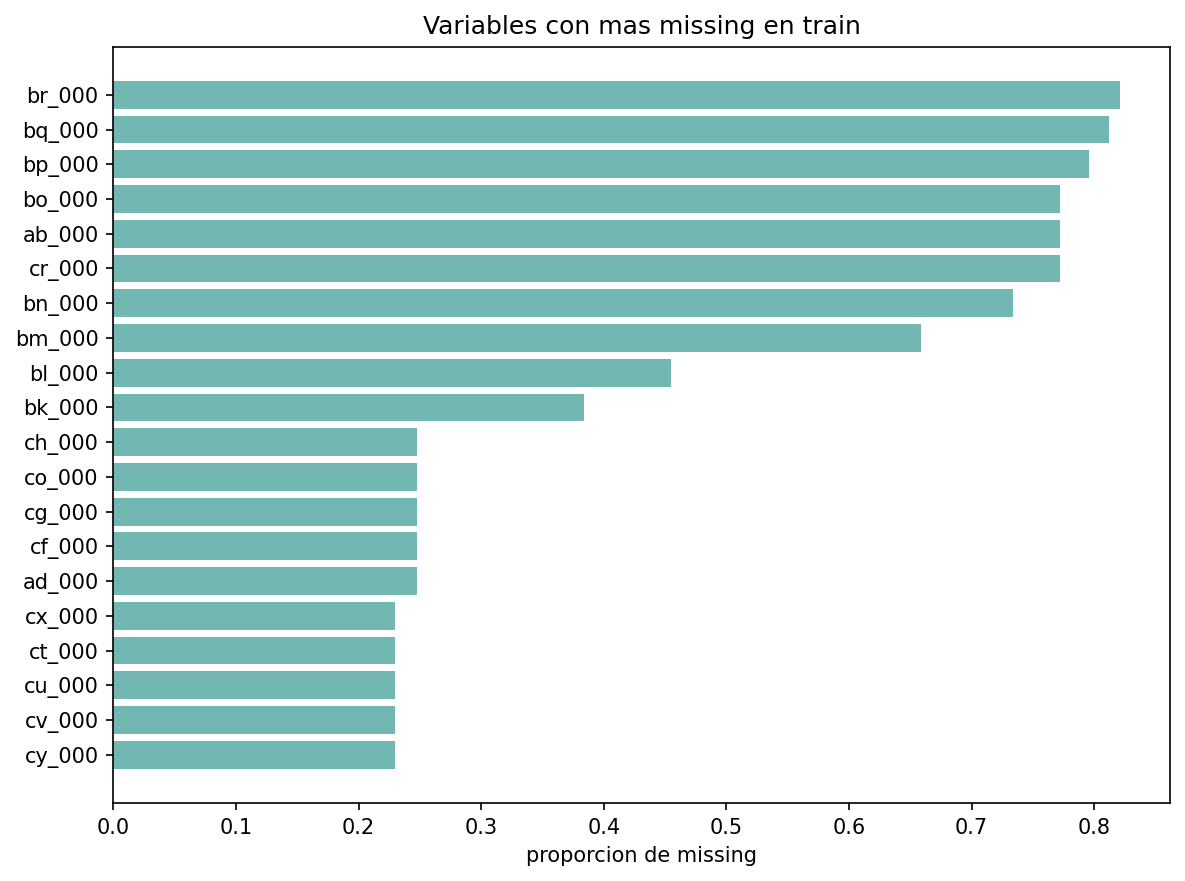
\includegraphics[width=0.82\textwidth]{missing_values_top30.png}
\caption{Variables con mayor proporción de valores faltantes en train}
\label{fig_missing}
\end{figure}

La Figura \ref{fig_missing} muestra el porcentaje total de valores faltantes por variable en todo train. El eje horizontal representa una proporción entre 0 y 1. Por ejemplo, un valor de 0.8 significa que aproximadamente el 80\% de los registros de esa variable están vacíos. Esta figura permite ver qué columnas tienen más ausencia de datos en general.

Además del missing total, el EDA analiza si la ausencia de datos cambia según la clase. Esto es importante porque un valor faltante no siempre significa simplemente un error de registro. En datos de sensores, una variable puede faltar porque un sensor no se activó, porque una condición del sistema no se produjo o porque el proceso de captura no registró esa señal. Por eso, la ausencia de datos también puede aportar información indirecta sobre el estado del camión.

En algunas variables, como \texttt{ac\_000}, \texttt{ad\_000}, \texttt{ae\_000}, \texttt{af\_000} y \texttt{ak\_000}, los valores faltantes son más frecuentes en la clase positiva. En otras, como \texttt{br\_000}, \texttt{bq\_000}, \texttt{bp\_000}, \texttt{bo\_000} y \texttt{bn\_000}, la ausencia aparece mucho más en la clase negativa.

\begin{figure}[H]
\centering
\includegraphics[width=0.78\textwidth]{missing_by_class_top20.png}
\caption{Variables con mayor diferencia de valores faltantes entre clases}
\label{fig_missing_clase}
\end{figure}

La Figura \ref{fig_missing_clase} no muestra el missing total, sino la diferencia máxima de missing entre clases. Su eje horizontal también es una proporción entre 0 y 1. Por ejemplo, una diferencia de 0.7 significa que la proporción de missing entre negativos y positivos cambia en unos 70 puntos porcentuales. Esta figura permite ver qué variables están vacías de forma distinta según la clase.

La lectura conjunta de ambas figuras es importante. La primera muestra qué columnas están más incompletas. La segunda muestra si esa ausencia está repartida de forma desigual entre negativos y positivos. Por tanto, los missing values no son solo un problema de limpieza, sino una característica relevante de la estructura del dataset.

Por este motivo, no se eliminan columnas de forma manual desde el EDA. Esa decisión podría descartar información útil o introducir criterios difíciles de justificar. En su lugar, los valores faltantes se tratan mediante imputación con mediana dentro de cada \texttt{Pipeline}. Así, durante la validación cruzada, cada fold calcula la mediana solo con su parte de entrenamiento y se evita fuga de información.

\subsubsection{Escalas, outliers y correlaciones}

Las variables tienen escalas muy diferentes. Algunas se concentran cerca de cero y otras alcanzan valores muy altos. También aparecen valores extremos. Según el análisis IQR, variables como \texttt{az\_007}, \texttt{dr\_000}, \texttt{dq\_000}, \texttt{bn\_000}, \texttt{ba\_008}, \texttt{cj\_000} y \texttt{aj\_000} tienen tasas elevadas de outliers.

\begin{figure}[H]
\centering
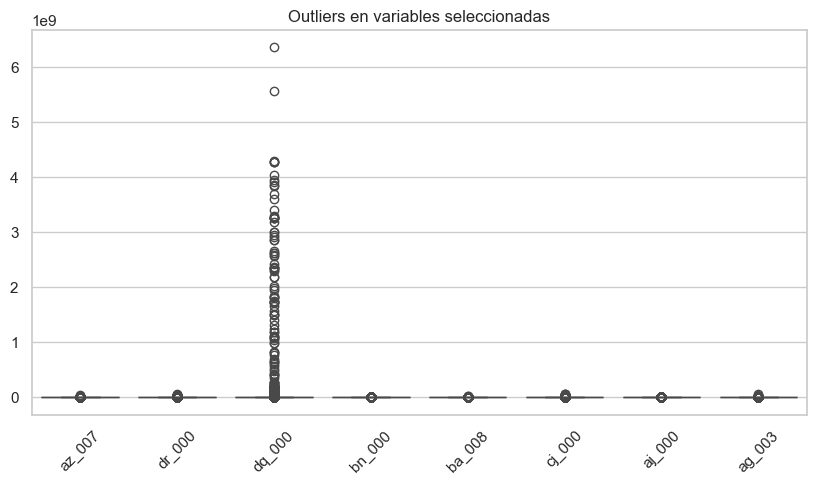
\includegraphics[width=0.82\textwidth]{boxplots_selected_variables.png}
\caption{Boxplots de variables seleccionadas para revisar escalas y valores extremos}
\label{fig_boxplots}
\end{figure}

La Figura \ref{fig_boxplots} ilustra la diferencia de escalas y la presencia de valores extremos en algunas variables. La visualización no es completamente cómoda porque \texttt{dq\_000} alcanza valores mucho más altos que el resto y comprime visualmente las demás distribuciones. Aun así, esta evidencia justifica el escalado en modelos sensibles a la magnitud de las variables y la comparación con modelos basados en árboles.

Para complementar esa visualización, la Tabla \ref{tab_outliers_iqr_resumen} resume las variables con mayor proporción de outliers según la regla IQR.

\begin{table}[H]
\centering
\caption{Ejemplos de variables con mayor proporción de outliers según la regla IQR}
\label{tab_outliers_iqr_resumen}
\small
\begin{tabular}{@{}lrrrr@{}}
\toprule
\textbf{Variable} & \textbf{Outliers} & \textbf{Tasa} & \textbf{Q1} & \textbf{Q3}\\
\midrule
\texttt{az\_007} & 14235 & 0.240 & 0 & 0\\
\texttt{dr\_000} & 13007 & 0.227 & 0 & 0\\
\texttt{dq\_000} & 12870 & 0.225 & 0 & 0\\
\texttt{bn\_000} & 3509 & 0.219 & 171720 & 493100\\
\texttt{ba\_008} & 12580 & 0.212 & 0 & 1820\\
\texttt{cj\_000} & 12540 & 0.210 & 0 & 0\\
\texttt{aj\_000} & 12452 & 0.210 & 0 & 0\\
\texttt{ag\_003} & 12435 & 0.210 & 0 & 0\\
\texttt{dy\_000} & 11867 & 0.207 & 0 & 36\\
\texttt{dx\_000} & 11572 & 0.202 & 0 & 8764\\
\bottomrule
\end{tabular}
\end{table}

La tabla muestra que los valores extremos no se concentran en una única variable. Varias columnas tienen más de un 20\% de registros considerados outliers por la regla IQR. En muchas de ellas, como \texttt{az\_007}, \texttt{dr\_000}, \texttt{dq\_000}, \texttt{cj\_000}, \texttt{aj\_000} y \texttt{ag\_003}, tanto Q1 como Q3 son 0. Esto significa que la mayoría de registros están concentrados en cero, pero existe un grupo relevante de casos con valores distintos y alejados de ese comportamiento habitual.

Este patrón es razonable en datos industriales. Algunas señales pueden permanecer inactivas durante funcionamiento normal y activarse solo en condiciones concretas. Por eso no se eliminan estos valores automáticamente. Pueden representar información útil sobre estados anómalos del camión y ayudan a justificar el uso de modelos capaces de manejar distribuciones asimétricas y con colas largas.

Las correlaciones muestran redundancia entre algunas variables. Por ejemplo, \texttt{aa\_000} y \texttt{bt\_000} tienen una correlación prácticamente perfecta en la muestra analizada. También aparecen relaciones altas entre \texttt{ci\_000}, \texttt{ao\_000}, \texttt{bj\_000}, \texttt{bi\_000} y otras variables. Esta redundancia es habitual en datos de sensores.

\begin{figure}[H]
\centering
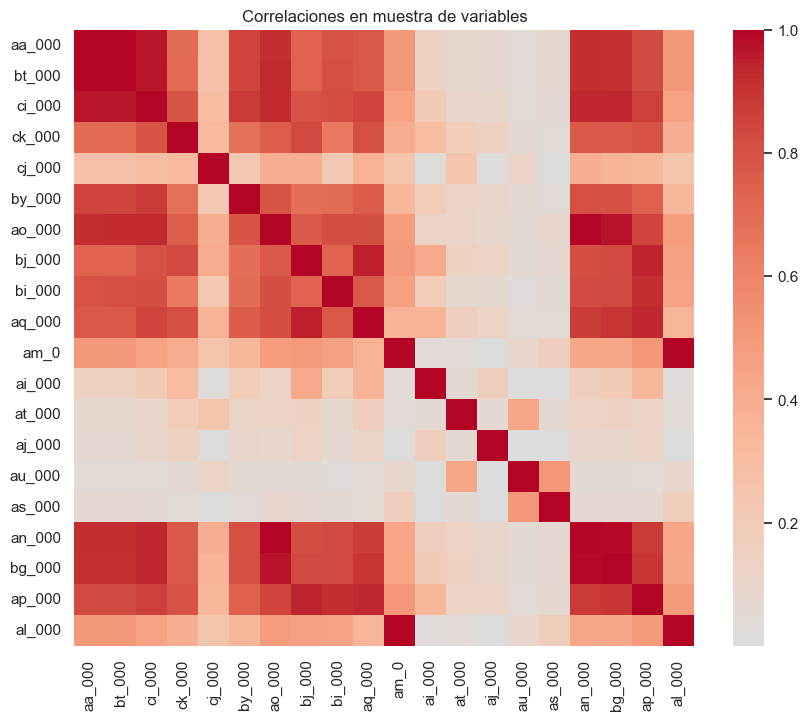
\includegraphics[width=0.72\textwidth]{correlation_sample_train.png}
\caption{Matriz de correlaciones en una selección de variables numéricas}
\label{fig_correlaciones}
\end{figure}

La Figura \ref{fig_correlaciones} confirma que algunas señales están muy relacionadas. Esta redundancia no se elimina manualmente, porque puede ser propia de datos de sensores y cada familia de modelos puede gestionarla de forma distinta.

Estas observaciones motivan el uso de escalado en modelos sensibles a escala, como regresión logística y SVM lineal. Los modelos basados en árboles no necesitan el mismo tratamiento, aunque todos mantienen imputación dentro del pipeline.

\subsection{Problemáticas identificadas}
\label{sec_problematicas}

En este proyecto se identifican varias problemáticas reales asociadas al uso de sistemas de aprendizaje automático en mantenimiento predictivo.

El primer problema es el desbalanceo de clase. La clase positiva es minoritaria y representa aproximadamente el 1.67\% de train. Esto implica que un modelo puede acertar muchos negativos y aun así fallar en el objetivo real del sistema, que es detectar fallos APS. Por este motivo se usan PR-AUC, recall positivo, F1 positivo, balanced accuracy y coste, en lugar de depender solo de accuracy.

El segundo problema son los datos escasos en la clase positiva. Aunque el dataset tiene 60000 filas de train, los casos APS son pocos en términos relativos. Esto dificulta aprender la frontera de decisión de la clase de interés y hace que cada falso negativo tenga importancia. La comparación con el baseline permite comprobar si los modelos aprenden señal útil o si solo reflejan la clase mayoritaria.

El tercer problema es el coste asimétrico. En el dominio de mantenimiento, revisar un camión sin fallo no tiene el mismo impacto que dejar pasar una avería real. El dataset formaliza esta diferencia con coste 10 para falsos positivos y 500 para falsos negativos. Por eso se estudia una estrategia alternativa, \texttt{logistic\_class\_weight}, que reduce falsos negativos aunque aumente falsas alarmas.

El cuarto problema es la explicabilidad. Aunque las variables están anonimizadas y no permiten una interpretación física directa, la explicabilidad sigue siendo útil. La importancia por permutación permite identificar qué señales influyen más en el rendimiento del modelo, detectar dependencias excesivas de variables concretas y orientar una revisión posterior con expertos de mantenimiento. Por tanto, la explicación no se interpreta como causalidad, sino como una auditoría del comportamiento predictivo del modelo.

El quinto problema es la robustez. En un sistema industrial, las señales pueden variar por ruido, cambios de sensores o condiciones de registro. La prueba con ruido no es una evaluación final nueva, sino una auditoría de sensibilidad que permite observar si el modelo se degrada ante perturbaciones de entrada.

El sexto problema es el shift o posible drift. El dataset no proporciona una validación temporal de producción, pero comparar train y test ayuda a revisar si las distribuciones son parecidas. En un despliegue real, esta dimensión sería crítica porque los camiones, sensores y patrones de mantenimiento pueden cambiar con el tiempo.

El séptimo problema son las anomalías. Los fallos APS pueden entenderse parcialmente como casos raros respecto al funcionamiento normal. Por eso se estudian detectores de anomalías como análisis auxiliar. Este enfoque no sustituye al modelo supervisado, pero puede aportar señales de alerta complementarias.

Fairness y privacidad no son el foco principal del proyecto porque las variables están anonimizadas y no hay atributos sensibles interpretables como sexo, edad, raza o grupo social. Esto impide analizar equidad por grupos de forma responsable. Aun así, la anonimización también limita la interpretación física. En un contexto interno de Scania, conocer el significado real de las variables permitiría validar mejor las explicaciones del modelo con expertos.

\subsection{Flujo reproducible de notebooks}
\label{sec_flujo_notebooks}

El proyecto está organizado como un flujo de notebooks numerados. El notebook \texttt{00\_descarga\_y\_\allowbreak preparacion.ipynb} descarga o carga el dataset, convierte los valores \texttt{na}, codifica la variable objetivo y guarda las particiones procesadas. Este paso fija la base común para el resto del trabajo.

El notebook \texttt{01\_EDA.ipynb} identifica las principales dificultades del dataset. En él se analiza la distribución de clases, los valores faltantes, las diferencias de missing por clase, las escalas, los outliers y las correlaciones. Estas observaciones justifican las decisiones metodológicas posteriores.

El notebook \texttt{02\_modelado\_\allowbreak supervisado.ipynb} contiene el modelado principal. Compara el baseline y los modelos supervisados mediante \texttt{GridSearchCV}, 5-fold CV y \texttt{Pipeline}. La selección del modelo principal se realiza solo con train.

El notebook \texttt{03\_desbalanceo\_\allowbreak y\_\allowbreak coste.ipynb} estudia estrategias sensibles al desbalanceo y al coste. Su función no es cambiar el modelo final mirando test, sino analizar el intercambio entre PR-AUC, recall, falsos positivos, falsos negativos y coste.

El notebook \texttt{04\_anomalias.ipynb} analiza detectores de anomalías entrenados sobre casos normales de train. Este análisis queda separado del modelo supervisado y se interpreta como una alerta secundaria.

El notebook \texttt{05\_xai\_\allowbreak robustez\_\allowbreak errores.ipynb} audita el modelo principal con importancia por permutación, análisis de errores, robustez ante ruido y shift entre train y test. No modifica hiperparámetros, umbrales ni la selección del modelo.

\section{Metodología}
\label{sec_metodologia}

\subsection{Conceptos técnicos usados}
\label{sec_conceptos}

Antes de describir el protocolo experimental conviene aclarar varios conceptos que aparecen a lo largo de la memoria. Un \texttt{Pipeline} es una cadena de pasos que aplica siempre el mismo preprocesamiento y el mismo modelo. En este proyecto permite que la imputación de valores faltantes, el escalado cuando procede y el clasificador se entrenen como una unidad. Esto es importante porque evita que información de validación o test se use accidentalmente durante el ajuste.

\texttt{GridSearchCV} es una búsqueda sistemática de hiperparámetros. Para cada combinación propuesta, el método entrena y valida el modelo varias veces usando validación cruzada. La validación cruzada de 5 folds divide train en cinco partes. En cada repetición, cuatro partes se usan para entrenar y una para validar. El resultado final es una media de rendimiento más estable que una única partición interna.

El término \textit{refit} indica que, una vez elegida la mejor configuración con validación cruzada, el estimador se vuelve a entrenar usando todo train. Así se aprovechan todos los datos de entrenamiento antes de evaluar en test. En este proyecto, test solo se usa después de este paso.

El baseline es un modelo de referencia simple. Sirve para comprobar si los modelos más complejos aportan valor real. Si un modelo avanzado no mejora claramente al baseline, no habría evidencia sólida de aprendizaje útil.

\texttt{HistGradientBoosting} es un modelo de boosting basado en árboles. Construye varios árboles de forma secuencial, de modo que cada nuevo árbol intenta corregir errores de los anteriores. Suele funcionar bien en datos tabulares porque puede capturar relaciones no lineales e interacciones entre variables.

La importancia por permutación es una técnica de explicabilidad global. Consiste en desordenar una variable y medir cuánto empeora la métrica del modelo. Si al desordenar una variable cae mucho la PR-AUC, esa variable es importante para el comportamiento predictivo. Esta técnica no demuestra causalidad. Solo indica dependencia estadística del modelo.

El análisis de anomalías busca observaciones raras respecto a un patrón normal. En este trabajo se entrena con casos negativos de train para comprobar si los fallos APS aparecen como casos anómalos. Es un análisis auxiliar, porque el objetivo principal sigue siendo la clasificación supervisada.

La robustez mide la sensibilidad del modelo ante cambios en la entrada. Aquí se añade ruido a variables numéricas para observar si el rendimiento se degrada. Esta prueba no sustituye a test ni cambia el modelo. Su función es auditar si el sistema depende de señales muy estables.

El shift o posible drift se refiere a cambios en la distribución de los datos. Shift describe diferencias entre particiones, como train y test. Drift suele usarse cuando ese cambio ocurre con el tiempo en producción. El dataset no permite afirmar deriva temporal estricta, pero sí permite comparar si train y test tienen distribuciones parecidas.

\subsection{Protocolo experimental}

El protocolo experimental es una parte central del proyecto. La partición oficial de train se usa para explorar, entrenar y seleccionar modelos. La partición oficial de test se reserva para la evaluación final. El test no se usa para ajustar hiperparámetros, no ajusta umbrales, no elige modelo y no elige estrategia.

Los modelos se comparan con \texttt{GridSearchCV} y validación cruzada estratificada de 5 folds sobre train. El preprocesamiento forma parte de \texttt{Pipeline}, por lo que la imputación y el escalado se ajustan dentro de cada fold. Esto evita fuga de información desde validación hacia entrenamiento.

Después de la búsqueda, \texttt{GridSearchCV} reentrena el mejor estimador con todo train mediante \texttt{refit}. Solo entonces se evalúa en test. Las tablas de test se interpretan como comparación final o como auditoría posterior, nunca como criterio de selección.

\subsection{Modelos comparados}

La Tabla \ref{tab_modelos} resume los modelos supervisados comparados.

\begin{table}[H]
\centering
\caption{Modelos supervisados comparados}
\label{tab_modelos}
\small
\begin{tabular}{@{}lp{0.62\textwidth}@{}}
\toprule
\textbf{Familia} & \textbf{Modelos}\\
\midrule
Baseline & \texttt{DummyClassifier}\\
Modelos lineales & Regresión logística y SVM lineal\\
Árbol simple & Árbol de decisión\\
Ensembles & Random Forest, Extra Trees, AdaBoost e HistGradientBoosting\\
\bottomrule
\end{tabular}
\end{table}

Todos los modelos usan imputación con mediana dentro del \texttt{Pipeline}, excepto \texttt{HistGradientBoosting}, que gestiona los valores faltantes de forma nativa y por tanto no necesita un paso previo de imputación. La regresión logística y la SVM lineal incorporan además \texttt{StandardScaler}. La métrica principal de selección es \texttt{average\_precision}, equivalente a PR-AUC. Como métricas complementarias se reportan recall positivo, F1 positivo, balanced accuracy, ROC-AUC y coste.

\subsection{Métricas de evaluación}
\label{sec_metricas}

Las métricas se eligen teniendo en cuenta el desbalanceo y el coste operativo de los errores. La \textit{accuracy} mide la proporción total de aciertos, pero puede ser engañosa porque la clase negativa domina el dataset. Por eso se usa solo como referencia general y no como criterio principal.

La \textit{precisión positiva} mide qué proporción de las predicciones positivas son realmente fallos APS. Es útil para estimar cuántas alertas generadas por el sistema serían correctas. El \textit{recall positivo} mide qué proporción de fallos APS reales se detectan. En este proyecto es especialmente importante porque un falso negativo implica dejar pasar un fallo real.

El \textit{F1 positivo} combina precisión y recall de la clase positiva mediante su media armónica. Esta métrica resume el equilibrio entre generar alertas correctas y detectar suficientes fallos APS. La \textit{balanced accuracy} promedia el rendimiento por clase y es más informativa que accuracy cuando hay desbalanceo.

La \textit{ROC-AUC} mide la capacidad de ranking del modelo considerando la relación entre verdaderos positivos y falsos positivos a distintos umbrales. La \textit{PR-AUC}, implementada como \texttt{average\_precision}, resume la curva precisión-recall. Es la métrica principal de selección porque se centra en la clase positiva minoritaria y es más adecuada cuando los positivos son escasos.

El coste se calcula con la expresión de la Ecuación \ref{eq_coste}.

\begin{equation}
\label{eq_coste}
C = 10 \cdot FP + 500 \cdot FN
\end{equation}

\subsection{Reproducibilidad}
\label{sec_reproducibilidad}

La reproducibilidad se apoya en cuatro decisiones. La primera es la separación de responsabilidades entre notebooks. Cada etapa produce artefactos que la siguiente puede cargar, lo que evita depender de resultados manuales. La segunda es la estructura de carpetas automatizada mediante la función \texttt{crear\_carpetas} de \texttt{project\_utils.py}, que genera de forma programática los directorios \texttt{data/raw}, \texttt{data/processed}, \texttt{artifacts/metrics}, \texttt{artifacts/models}, \texttt{artifacts/figures} y \texttt{artifacts/tables}, garantizando que cualquier ejecución parta de una organización de archivos consistente. La tercera es el uso de funciones comunes en \texttt{project\_utils.py}. Este módulo define la carga del dataset, la conversión de etiquetas, el cálculo de métricas, la matriz de confusión y el coste. La cuarta es la fijación de \texttt{RANDOM\_STATE = 42} en todos los experimentos, lo que asegura que los resultados sean deterministas y reproducibles ante cualquier re-ejecución.

El entorno se documenta en \texttt{requirements.txt}. Las dependencias principales son \texttt{numpy}, \texttt{pandas}, \texttt{scikit-learn}, \texttt{matplotlib}, \texttt{seaborn}, \texttt{joblib}, \texttt{ucimlrepo}, \texttt{notebook} y \texttt{nbconvert}. El repositorio incluye un \texttt{README.md} con instrucciones de instalación y orden de ejecución. Esto permite reconstruir el flujo desde una máquina limpia, siempre que los datos o su descarga estén disponibles.

Desde el punto de vista experimental, la reproducibilidad también exige no usar test durante la toma de decisiones. Por ello, las tablas de test se generan una vez fijados modelos, hiperparámetros y estrategias. Cualquier ajuste futuro de coste o umbral debería hacerse con validación interna en train, no con test.

\section{Experimentos y resultados}
\label{sec_experimentos}

\subsection{Modelado supervisado}
\label{sec_modelado}

\subsubsection{Resultados de validación cruzada}

La Tabla \ref{tab_cv} muestra los resultados medios de validación cruzada sobre train. La tabla está ordenada por PR-AUC, que es la métrica principal de selección.

\begin{table}[H]
\centering
\caption{Comparativa de modelos con 5-fold CV sobre train}
\label{tab_cv}
\small
\begin{tabular}{@{}lrrrrr@{}}
\toprule
\textbf{Modelo} & \textbf{PR-AUC} & \textbf{Recall pos.} & \textbf{F1 pos.} & \textbf{Bal. acc.} & \textbf{Tiempo s}\\
\midrule
\rowcolor{bestrow} HistGradientBoosting & \textbf{0.881} & 0.738 & \textbf{0.809} & \textbf{0.868} & 35.9\\
Random Forest & 0.874 & 0.697 & 0.787 & 0.848 & 145.5\\
Extra Trees & 0.865 & 0.702 & 0.793 & 0.850 & 34.2\\
AdaBoost & 0.794 & 0.665 & 0.730 & 0.831 & 172.3\\
Logistic Regression & 0.772 & 0.632 & 0.708 & 0.815 & 31.3\\
Linear SVM & 0.769 & 0.619 & 0.708 & 0.808 & 1328.0\\
Decision Tree & 0.706 & 0.639 & 0.698 & 0.818 & 50.0\\
\rowcolor{worstrow} Dummy & 0.017 & 0.021 & 0.021 & 0.502 & 5.0\\
\bottomrule
\end{tabular}
\end{table}

El baseline confirma que una estrategia simple casi no detecta positivos. El modelo \texttt{Dummy} obtiene una PR-AUC de 0.017 y un recall positivo de 0.021, por lo que sirve para mostrar que la accuracy no sería una métrica suficiente en este problema. Frente a esta referencia, todos los modelos entrenados aprenden señal útil del dataset.

\texttt{HistGradientBoosting} obtiene el mejor resultado global, con una PR-AUC media de 0.881 y el mejor F1 positivo, con 0.809. Esto lo convierte en el modelo seleccionado según la métrica principal. Sin embargo, la diferencia con otros ensembles no es extrema. \texttt{Random Forest} alcanza una PR-AUC de 0.874 y queda como segundo mejor modelo, aunque tarda 145.5 segundos, bastante más que \texttt{HistGradientBoosting}. \texttt{Extra Trees} también es una alternativa competitiva, con PR-AUC de 0.865, F1 positivo de 0.793 y un tiempo de 34.2 segundos, muy similar al modelo seleccionado.

Los modelos lineales ofrecen una referencia útil, pero quedan por debajo de los ensembles. \texttt{Logistic Regression} obtiene una PR-AUC de 0.772 con un tiempo bajo, lo que la convierte en un modelo simple y razonable como comparación. En cambio, \texttt{Linear SVM} no resulta eficiente en este experimento, ya que tarda alrededor de 1328 segundos y no mejora a la regresión logística ni a los ensembles.

En conjunto, la comparación muestra que \texttt{HistGradientBoosting} ofrece el mejor equilibrio entre rendimiento y coste computacional. \texttt{Random Forest} es muy competitivo, pero más lento. \texttt{Extra Trees} destaca como alternativa rápida y sólida. Los modelos lineales y el árbol simple son útiles como referencia, pero no alcanzan el rendimiento de los ensembles principales.

\subsubsection{Selección del modelo principal}

El modelo principal es \texttt{hist\_gradient\_boosting}. La selección se hace solo con validación cruzada en train y usando PR-AUC. El valor de selección guardado en los artefactos es 0.881018. Esta decisión se toma antes de analizar el rendimiento final en test.

\subsection{Resultados finales en test}
\label{sec_test}

Una vez seleccionado el modelo principal, se evalúa en test. La Tabla \ref{tab_test} muestra la comparativa final de los modelos ya ajustados.

\begin{table}[H]
\centering
\caption{Comparativa final en test}
\label{tab_test}
\small
\begin{tabular}{@{}lrrrrrr@{}}
\toprule
\textbf{Modelo} & \textbf{PR-AUC} & \textbf{Recall pos.} & \textbf{F1 pos.} & \textbf{FP} & \textbf{FN} & \textbf{Coste}\\
\midrule
\rowcolor{bestrow} HistGradientBoosting & \textbf{0.922} & \textbf{0.752} & \textbf{0.842} & \textbf{13} & \textbf{93} & \textbf{46630}\\
Random Forest & 0.920 & 0.717 & 0.816 & 15 & 106 & 53150\\
Extra Trees & 0.918 & 0.704 & 0.805 & 17 & 111 & 55670\\
AdaBoost & 0.840 & 0.680 & 0.753 & 47 & 120 & 60470\\
Logistic Regression & 0.819 & 0.701 & 0.767 & 48 & 112 & 56480\\
Linear SVM & 0.822 & 0.645 & 0.746 & 32 & 133 & 66820\\
Decision Tree & 0.770 & 0.645 & 0.748 & 30 & 133 & 66800\\
Dummy & 0.024 & 0.016 & 0.018 & 272 & 369 & 187220\\
\bottomrule
\end{tabular}
\end{table}

La Tabla \ref{tab_test} confirma que el comportamiento observado en validación cruzada se mantiene en test. \texttt{HistGradientBoosting} obtiene el mejor resultado global, con PR-AUC de 0.922, F1 positivo de 0.842 y recall positivo de 0.752. Por eso se mantiene como modelo principal.

Otros ensembles, como \texttt{Random Forest} y \texttt{Extra Trees}, no quedan muy lejos y también muestran un rendimiento sólido. Sin embargo, \texttt{HistGradientBoosting} combina mejor PR-AUC, F1 positivo, menor número de falsos positivos y menor coste entre los modelos supervisados principales.

El baseline vuelve a quedar muy por debajo, lo que confirma que el problema requiere modelos capaces de aprender patrones reales en las variables. La matriz de confusión del modelo seleccionado se muestra en la Figura \ref{fig_confusion}.

\begin{figure}[H]
\centering
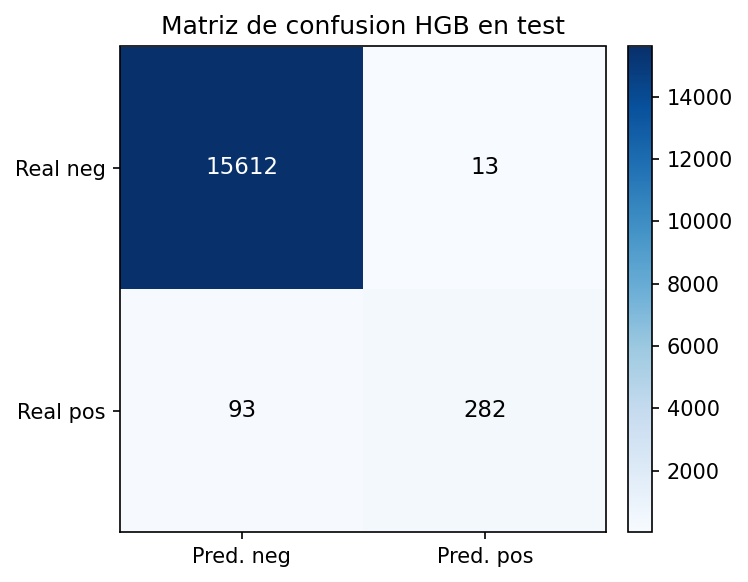
\includegraphics[width=0.58\textwidth]{confusion_matrix_best_model.png}
\caption{Matriz de confusión del modelo \texttt{HistGradientBoosting} en test}
\label{fig_confusion}
\end{figure}

La Figura \ref{fig_confusion} resume visualmente los aciertos y errores del modelo final. La diagonal principal representa las predicciones correctas. En ella aparecen los verdaderos negativos y los verdaderos positivos. El modelo clasifica correctamente 15612 casos negativos y detecta 282 fallos APS.

Los errores aparecen fuera de esa diagonal. Hay 13 falsos positivos, que son camiones marcados como fallo APS aunque no lo eran, y 93 falsos negativos, que son fallos APS reales que el modelo no detecta. Estos últimos son el punto más delicado porque tienen mayor impacto operativo.

\subsection{Desbalanceo y coste}
\label{sec_coste}

El notebook de desbalanceo y coste no sustituye al modelo principal. Su función es estudiar cómo cambian las métricas cuando se introducen estrategias sensibles al desbalanceo. Las estrategias comparadas son \texttt{hgb\_sin\_ajuste}, \texttt{logistic\_sin\_ajuste}, \texttt{logistic\_class\_weight} y \texttt{rf\_class\_weight}. Se decidió evaluar deliberadamente la versión de \texttt{HistGradientBoosting} sin ajuste específico para el desbalanceo ---una configuración a priori en desventaja frente a las estrategias que sí incorporan modificaciones explícitas como \texttt{class\_weight}--- para demostrar cómo, gracias a su naturaleza intrínseca de entrenamiento y robustez, el modelo sigue siendo capaz de superar a las demás alternativas incluso sin adaptaciones al coste asimétrico.

La selección por PR-AUC en validación cruzada sobre el conjunto de entrenamiento (train) vuelve a elegir \texttt{hgb\_sin\_ajuste}, con una PR-AUC media de 0.881 obtenida estrictamente en dicha validación cruzada. La Tabla \ref{tab_coste} muestra la comparación final en test de estas estrategias.

\begin{table}[H]
\centering
\caption{Comparativa de estrategias de desbalanceo y coste en test}
\label{tab_coste}
\small
\begin{tabular}{@{}lrrrrrr@{}}
\toprule
\textbf{Estrategia} & \textbf{PR-AUC} & \textbf{Recall pos.} & \textbf{F1 pos.} & \textbf{FP} & \textbf{FN} & \textbf{Coste}\\
\midrule
\rowcolor{bestrow} \texttt{hgb\_sin\_ajuste} & 0.922 & 0.752 & \textbf{0.842} & \textbf{13} & 93 & 46630\\
\texttt{rf\_class\_weight} & 0.880 & 0.573 & 0.712 & 14 & 160 & 80140\\
\texttt{logistic\_sin\_ajuste} & 0.819 & 0.701 & 0.767 & 48 & 112 & 56480\\
\rowcolor{altrow} \texttt{logistic\_class\_weight} & 0.800 & \textbf{0.925} & 0.639 & 364 & \textbf{28} & \textbf{17640}\\
\bottomrule
\end{tabular}
\end{table}

\texttt{logistic\_class\_weight} reduce los falsos negativos de 93 a 28. A cambio aumenta los falsos positivos de 13 a 364 y reduce F1 positivo. Como el coste penaliza mucho más los falsos negativos, su coste total baja a 17640 frente a 46630 de \texttt{HistGradientBoosting}.

Este resultado no cambia el modelo principal. La razón es metodológica. El modelo principal se seleccionó por PR-AUC en train antes de mirar test. Si el objetivo principal fuese minimizar coste, habría que diseñar un experimento donde el coste se optimizara dentro de train mediante validación cruzada. No sería correcto escoger \texttt{logistic\_class\_weight} como modelo final solo porque su coste en test sea menor.

\subsection{Análisis de anomalías}
\label{sec_anomalias}

El análisis de anomalías es secundario y no sustituye al modelo supervisado. Su objetivo es comprobar si los fallos APS aparecen como observaciones raras frente a los casos normales. En este contexto, un detector de anomalías es un modelo que aprende cómo son los casos normales y asigna una puntuación de rareza a cada nueva observación.

Los detectores se entrenan con casos normales de train. Después, los casos que se alejan más de ese comportamiento normal se marcan como posibles anomalías. Los umbrales se calculan usando train y test se utiliza solo para evaluar. Se comparan Isolation Forest, Local Outlier Factor y One-Class SVM. La Tabla \ref{tab_anomalias} resume los resultados.

\begin{figure}[H]
\centering
\includegraphics[width=0.72\textwidth]{anomaly_scores_isolation_forest.png}
\caption{Comparación de recall positivo y falsos positivos en detectores de anomalías}
\label{fig_anomalias}
\end{figure}

La Figura \ref{fig_anomalias} muestra el intercambio principal de los detectores de anomalías. One-Class SVM alcanza el mayor recall positivo, pero también genera muchos más falsos positivos. Respecto a la comparativa global, la Tabla \ref{tab_anomalias} resume los resultados de los detectores en test.

\begin{table}[H]
\centering
\caption{Resultados de detección de anomalías en test}
\label{tab_anomalias}
\small
\begin{tabular}{@{}lrrrrrr@{}}
\toprule
\textbf{Detector} & \textbf{PR-AUC} & \textbf{Recall pos.} & \textbf{F1 pos.} & \textbf{FP} & \textbf{FN} & \textbf{Coste}\\
\midrule
Isolation Forest & 0.568 & 0.699 & 0.604 & 231 & 113 & 58810\\
Local Outlier Factor & 0.146 & 0.181 & 0.185 & 291 & 307 & 156410\\
One-Class SVM & \textbf{0.589} & \textbf{0.899} & 0.519 & 586 & \textbf{38} & \textbf{24860}\\
\bottomrule
\end{tabular}
\end{table}

La Tabla \ref{tab_anomalias} no representa una nueva selección del modelo principal, sino una comparación secundaria con otro enfoque. A diferencia del clasificador supervisado, estos detectores no aprenden directamente a distinguir entre casos APS y no APS. Se entrenan con casos normales para aprender el comportamiento habitual del camión y después marcan como sospechosos los casos que se alejan de ese patrón.

Este análisis sirve para comprobar si un fallo APS también puede verse como un comportamiento raro del camión. Por eso los detectores de anomalías podrían usarse como una alerta auxiliar separada del modelo principal, pero no como sustituto directo.

En esta comparación, \texttt{One-Class SVM} detecta muchos positivos y reduce los falsos negativos a 38. Sin embargo, genera 586 falsos positivos. Esto significa que deja escapar menos fallos, pero también enviaría más camiones a revisión. Por tanto, puede ser útil si se quiere priorizar la detección, aunque implique aceptar más falsas alarmas.

\subsection{Explicabilidad, robustez y errores}
\label{sec_xai}

\subsubsection{Importancia por permutación}

La importancia por permutación se calcula sobre una muestra de train y mide cuánto cae average precision cuando se desordena una variable. Si al alterar una variable el rendimiento baja mucho, significa que el modelo dependía bastante de esa información para predecir. La Tabla \ref{tab_importancia} muestra las variables más influyentes.

\begin{figure}[H]
\centering
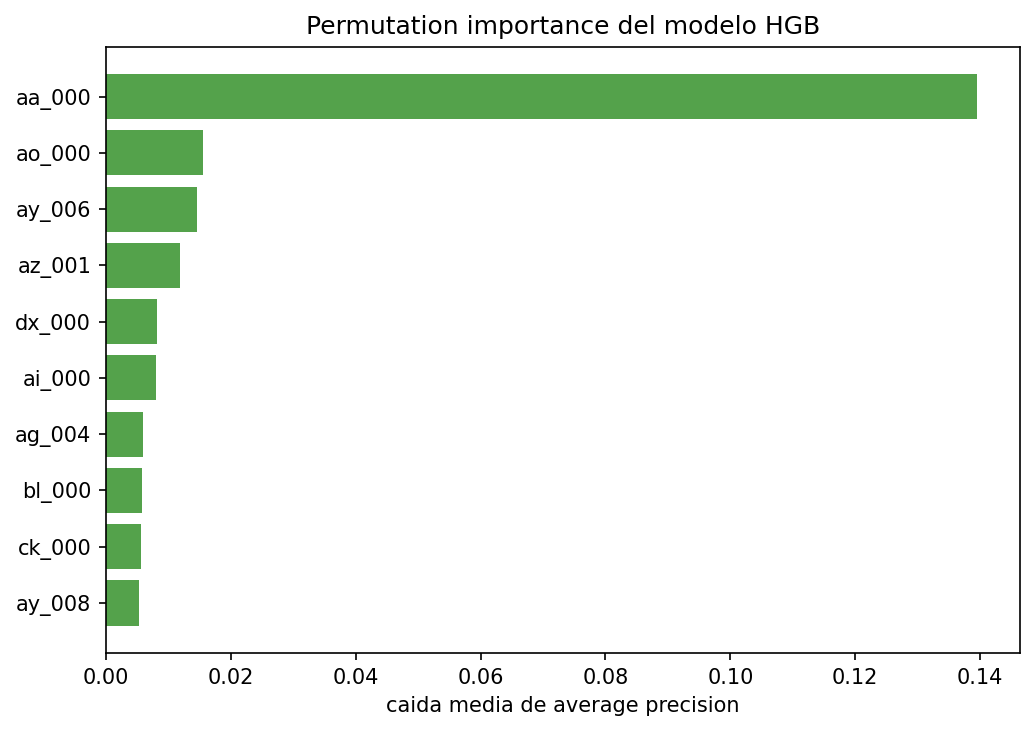
\includegraphics[width=0.78\textwidth]{feature_importance.png}
\caption{Importancia por permutación del modelo principal}
\label{fig_importancia}
\end{figure}

La Figura \ref{fig_importancia} permite ver que la importancia está muy concentrada. \texttt{aa\_000} destaca con mucha diferencia sobre el resto, lo que conviene tener en cuenta al interpretar la estabilidad del modelo.

\begin{table}[H]
\centering
\caption{Variables más importantes por permutation importance}
\label{tab_importancia}
\small
\begin{tabular}{@{}lrr@{}}
\toprule
\textbf{Variable} & \textbf{Importancia media} & \textbf{Desv.}\\
\midrule
\texttt{aa\_000} & 0.1394 & 0.0252\\
\texttt{ao\_000} & 0.0156 & 0.0013\\
\texttt{ay\_006} & 0.0145 & 0.0080\\
\texttt{az\_001} & 0.0118 & 0.0043\\
\texttt{dx\_000} & 0.0082 & 0.0041\\
\texttt{ai\_000} & 0.0080 & 0.0010\\
\texttt{ag\_004} & 0.0059 & 0.0063\\
\texttt{bl\_000} & 0.0059 & 0.0051\\
\texttt{ck\_000} & 0.0056 & 0.0006\\
\texttt{ay\_008} & 0.0054 & 0.0038\\
\bottomrule
\end{tabular}
\end{table}

\texttt{aa\_000} domina claramente el ranking. Al permutar esta variable, la average precision cae alrededor de 0.139, lo que indica que el modelo pierde bastante capacidad predictiva cuando esa información se desordena. La segunda variable, \texttt{ao\_000}, queda muy por debajo con una caída de 0.016, por lo que la importancia está muy concentrada en \texttt{aa\_000}.

Este resultado sugiere que el modelo depende mucho de una señal principal. Debido a la anonimización, no se puede interpretar \texttt{aa\_000} como una causa física del fallo APS. Aun así, la importancia por permutación sí permite auditar el comportamiento del modelo e identificar qué señales deberían revisarse con mayor atención si se conociera su significado real.

\subsubsection{Análisis de errores}

El análisis de errores del modelo final muestra 15894 aciertos, 93 falsos negativos y 13 falsos positivos sobre 16000 observaciones de test. Un ejemplo local revisado en el notebook corresponde a un falso negativo. El caso real es positivo, pero el modelo lo predice como negativo. En ese ejemplo se inspeccionan los valores de las diez variables más importantes para entender el error desde las señales globales del modelo.

\begin{figure}[H]
\centering
\includegraphics[width=0.62\textwidth]{error_summary.png}
\caption{Resumen de aciertos, falsos negativos y falsos positivos en test}
\label{fig_errores}
\end{figure}

La Figura \ref{fig_errores} resume la distribución general de aciertos y errores en test. Aunque los errores son pocos en relación con el tamaño total de la partición, la matriz de confusión permite concretar su impacto. El modelo produce 13 falsos positivos y 93 falsos negativos.

La principal limitación operativa sigue siendo el falso negativo. Cada uno de esos 93 casos representa un fallo APS real que el modelo no detecta. Esta diferencia es relevante porque, según la función de coste definida, un falso negativo pesa mucho más que un falso positivo.

\subsubsection{Robustez ante ruido}

La prueba de robustez añade ruido a variables numéricas en una muestra de train. Es una auditoría de sensibilidad posterior al modelado. La Tabla \ref{tab_robustez} resume la degradación observada.

\begin{figure}[H]
\centering
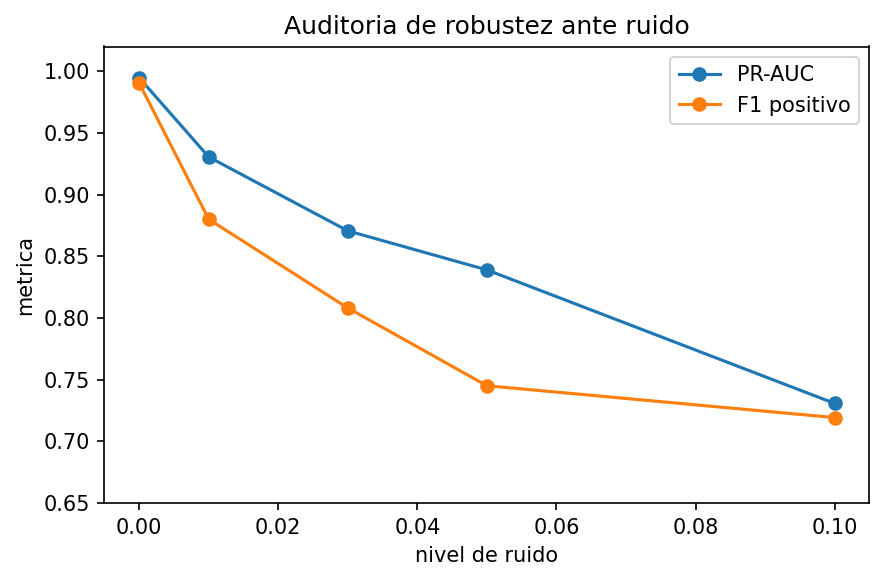
\includegraphics[width=0.72\textwidth]{robustness_curve.png}
\caption{Auditoría de sensibilidad ante ruido en variables numéricas}
\label{fig_robustez}
\end{figure}

La Figura \ref{fig_robustez} muestra una caída progresiva de PR-AUC y F1 positivo al aumentar el nivel de ruido. Con ruido bajo el modelo mantiene un rendimiento razonable, pero a medida que las variables se perturban más, ambas métricas descienden de forma clara. Esto indica que el modelo depende de la calidad de las señales de entrada. En un uso real sería importante monitorizar sensores, valores anómalos y cambios en la captura de datos para evitar una degradación del rendimiento.

\begin{table}[H]
\centering
\caption{Robustez ante ruido en variables numéricas}
\label{tab_robustez}
\small
\begin{tabular}{@{}rrrrrr@{}}
\toprule
\textbf{Ruido} & \textbf{PR-AUC} & \textbf{Recall pos.} & \textbf{F1 pos.} & \textbf{FP} & \textbf{FN}\\
\midrule
0.00 & 0.995 & 0.981 & 0.990 & 0 & 1\\
0.01 & 0.930 & 0.846 & 0.880 & 4 & 8\\
0.03 & 0.871 & 0.769 & 0.808 & 7 & 12\\
0.05 & 0.839 & 0.731 & 0.745 & 12 & 14\\
0.10 & 0.731 & 0.788 & 0.719 & 21 & 11\\
\bottomrule
\end{tabular}
\end{table}

La tabla complementa la figura anterior mostrando los mismos resultados con valores concretos. Se observa que al aumentar el ruido la PR-AUC baja de 0.995 a 0.731 y el F1 positivo baja de 0.990 a 0.719. Además, los falsos positivos aumentan de 0 a 21. Esto refuerza que el modelo es sensible a la calidad de las señales de entrada.

\subsubsection{Shift entre train y test}

El shift entre train y test se analiza con el estadístico KS por variable. Este estadístico compara si una misma variable tiene una distribución parecida en train y en test. En otras palabras, comprueba si los valores de una columna se reparten de forma similar en ambas particiones. Un valor KS cercano a 0 indica que las distribuciones son muy parecidas. Un valor más alto indicaría que esa variable se comporta de forma diferente en train y en test.

\begin{table}[H]
\centering
\caption{Variables con mayor diferencia de distribución entre train y test según KS}
\label{tab_shift_ks}
\small
\begin{tabular}{@{}lrr@{}}
\toprule
\textbf{Variable} & \textbf{KS} & \textbf{p-value}\\
\midrule
\texttt{br\_000} & 0.0227 & 0.1906\\
\texttt{bq\_000} & 0.0208 & 0.2515\\
\texttt{ab\_000} & 0.0152 & 0.5152\\
\texttt{bp\_000} & 0.0145 & 0.6432\\
\texttt{cz\_000} & 0.0124 & 0.1024\\
\texttt{cb\_000} & 0.0120 & 0.0555\\
\texttt{ay\_008} & 0.0118 & 0.0599\\
\texttt{bj\_000} & 0.0118 & 0.0597\\
\bottomrule
\end{tabular}
\end{table}

La Tabla \ref{tab_shift_ks} muestra las variables donde train y test se diferencian más según este estadístico. Aun así, los valores son bajos. La mayor diferencia aparece en \texttt{br\_000}, con KS de 0.0227, seguida de \texttt{bq\_000}, con 0.0208. Esto significa que incluso las variables más distintas tienen distribuciones bastante parecidas entre train y test.

El p-value ayuda a interpretar si la diferencia observada es estadísticamente clara. En las primeras variables, los p-values no son especialmente bajos, por lo que no hay evidencia fuerte de que train y test estén separados de forma importante en esas columnas.

La interpretación debe ser prudente. Este análisis no demuestra que no pueda haber deriva en producción, porque el dataset no representa un flujo temporal real. Solo permite comprobar que las particiones usadas en el proyecto parecen razonablemente parecidas desde el punto de vista distributivo.

\section{Discusión}
\label{sec_discusion}

\subsection{Por qué HistGradientBoosting es el modelo principal}

\texttt{HistGradientBoosting} es el modelo principal porque fue seleccionado por PR-AUC media en validación cruzada usando solo train. Además, mantiene el mejor rendimiento global en test entre los modelos comparados. Supera claramente al baseline, obtiene buen F1 positivo y genera muy pocos falsos positivos.

El resultado también es razonable desde el punto de vista técnico. Los modelos de boosting suelen funcionar bien en datos tabulares con relaciones no lineales e interacciones entre variables. En este proyecto, además, ofrece un buen equilibrio entre rendimiento y tiempo de entrenamiento.

\subsection{PR-AUC frente a coste}

PR-AUC y coste responden a preguntas distintas. PR-AUC evalúa la capacidad del modelo para ordenar positivos en un problema desbalanceado. El coste penaliza errores concretos con pesos distintos. Por eso \texttt{HistGradientBoosting} puede ser mejor por PR-AUC y \texttt{logistic\_class\_weight} puede ser mejor por coste en la comparativa final.

La conclusión correcta no es cambiar el modelo final mirando test. La lectura adecuada es que existe una alternativa operativa si el objetivo principal cambia. Para defender \texttt{logistic\_class\_weight} como modelo final habría que seleccionarlo dentro de train con una métrica de coste o con un protocolo de umbrales validado sin test.

Esta diferencia es importante para la toma de decisiones. Si el sistema se usa para priorizar revisiones con capacidad limitada, puede interesar un modelo con mayor precisión y pocas falsas alarmas. En ese caso, \texttt{HistGradientBoosting} ofrece un equilibrio razonable. Si el coste de dejar pasar fallos es muy alto y existe capacidad para revisar muchas alertas, una estrategia como \texttt{logistic\_class\_weight} puede ser más atractiva. La memoria separa ambas lecturas porque responden a objetivos operativos distintos.

\subsection{Explicabilidad con variables anonimizadas}

La explicabilidad tiene un papel particular en este dataset. Las variables no describen directamente componentes interpretables para una persona externa al fabricante. Por tanto, no se puede afirmar que una variable concreta sea la causa física del fallo. Aun así, la importancia por permutación aporta una lectura útil del comportamiento predictivo.

El resultado más relevante es la dependencia de \texttt{aa\_000}. Esta variable domina el ranking de importancia, lo que puede tener dos lecturas. Por un lado, puede ser una señal muy informativa para detectar fallos APS. Por otro lado, una dependencia excesiva de una sola señal puede aumentar la fragilidad si esa variable cambia, se registra mal o tiene un comportamiento distinto en producción.

La explicabilidad también ayuda a orientar una revisión posterior con expertos de mantenimiento. Un experto con acceso al significado real de las variables podría comprobar si las señales destacadas son coherentes con el funcionamiento del sistema APS. Además, el análisis de falsos positivos y falsos negativos permite revisar casos donde el modelo se equivoca y estudiar si el error se relaciona con patrones de variables importantes, missing values o condiciones anómalas.

\subsection{Limitaciones}

La primera limitación es la anonimización de variables. Se pueden detectar patrones estadísticos, pero no se puede explicar físicamente cada señal. La segunda limitación es el fuerte desbalanceo, que hace que pequeñas variaciones en falsos negativos tengan impacto relevante. La tercera limitación es el coste simplificado. La penalización de 10 y 500 es útil para comparar, pero no representa todos los costes reales de taller, logística y seguridad.

También hay limitaciones de evaluación. El proyecto usa una partición oficial de test, pero no valida el sistema en producción. No hay monitorización continua, validación temporal ni revisión por expertos de mantenimiento. Las pruebas de anomalías, robustez y shift son auditorías complementarias, no sustitutos de un despliegue real.

Fairness y privacidad se tratan como limitaciones de alcance. No se han identificado atributos sensibles interpretables, por lo que no se puede medir discriminación por grupos sociales. Tampoco se trabaja con datos personales directos en la memoria, ya que las variables están anonimizadas. Aun así, un despliegue real en una empresa debería revisar políticas de acceso, trazabilidad de alertas y gobierno de datos.

\subsection{Trabajo futuro}

Una mejora natural sería optimizar coste dentro de validación cruzada en train. Otra mejora sería estudiar umbrales de decisión con un conjunto de validación interno o validación cruzada, siempre sin usar test. También sería útil realizar validación temporal si se dispone de fechas, calibrar probabilidades y añadir revisión experta de falsos negativos.

En producción, sería necesario monitorizar drift, missing values, estabilidad de sensores, tasas de falsos negativos y coste real de intervención. También habría que diseñar una integración con procesos de mantenimiento y definir quién revisa las alertas.

\section{Conclusiones}
\label{sec_conclusiones}

El proyecto construye un flujo completo para detectar fallos APS en camiones Scania a partir de datos tabulares industriales. El dataset presenta dificultades reales como clase positiva minoritaria, valores faltantes, escalas diferentes, outliers, variables correlacionadas y anonimización.

Los modelos se comparan con \texttt{GridSearchCV}, 5-fold CV y \texttt{Pipeline}. La selección de hiperparámetros se hace solo con train. El mejor estimador se reentrena con todo train mediante \texttt{refit}. Test se usa solo para evaluación final y auditoría posterior. No elige modelo, estrategia, umbral ni hiperparámetros.

El modelo principal es \texttt{HistGradientBoosting}. Se selecciona por PR-AUC en train, obtiene PR-AUC cercana a 0.881 en validación cruzada y mantiene PR-AUC cercana a 0.922 en test. En la evaluación final alcanza F1 positivo cercano a 0.842 y recall positivo cercano a 0.752. La matriz de confusión muestra 15612 verdaderos negativos, 282 verdaderos positivos, 13 falsos positivos y 93 falsos negativos.

El análisis de coste muestra que los falsos negativos siguen siendo importantes. \texttt{logistic\_class\_weight} reduce los falsos negativos a 28 y baja el coste total a 17640, pero aumenta mucho los falsos positivos y no fue el modelo seleccionado por la métrica principal en train. Por tanto, queda como alternativa operativa y no como modelo final.

Los análisis de anomalías, explicabilidad, robustez, errores y shift aportan una visión más completa. Las anomalías sugieren que algunos fallos APS pueden comportarse como observaciones raras y podrían estudiarse como sistema auxiliar de alerta. La importancia por permutación muestra una dependencia fuerte de \texttt{aa\_000}. La robustez ante ruido evidencia sensibilidad a perturbaciones. El análisis de errores confirma que el modelo es útil, pero no perfecto.

En conjunto, el trabajo ofrece una solución técnica defendible para un problema real de mantenimiento predictivo. Su principal fortaleza no es solo el resultado de test, sino la separación estricta entre selección y evaluación, la comparación de modelos, la discusión de coste y la auditoría posterior del comportamiento.

\begin{table}[H]
\centering
\caption{Resumen final de conclusiones metodológicas}
\label{tab_conclusiones_metodologicas}
\small
\begin{tabular}{@{}p{0.32\textwidth}p{0.58\textwidth}@{}}
\toprule
\textbf{Aspecto} & \textbf{Conclusión}\\
\midrule
Modelo principal & \texttt{HistGradientBoosting}\\
Métrica de selección & PR-AUC media en 5-fold CV sobre train\\
Criterio metodológico & Selección con \texttt{GridSearchCV} y 5-fold CV en train. Test reservado solo para evaluación final\\
Mejor alternativa por coste & \texttt{logistic\_class\_weight}, con 28 falsos negativos y coste 17640 en test\\
Principal limitación & Variables anonimizadas, clase positiva minoritaria y coste simplificado\\
Trabajo futuro & Optimizar coste y umbrales dentro de train, validación temporal, calibración y revisión experta\\
\bottomrule
\end{tabular}
\end{table}

\section{Referencias}
\label{sec_referencias}

\renewcommand{\refname}{}
\vspace{-2.5em}

\begin{thebibliography}{9}

\bibitem{uciaps}
Dua, D. y Graff, C.
\newblock APS Failure at Scania Trucks.
\newblock UCI Machine Learning Repository.
\newblock University of California, Irvine, School of Information and Computer Sciences.
\newblock \url{https://archive.ics.uci.edu/dataset/421/aps+failure+at+scania+trucks}

\bibitem{apravanzado}
Lozano Ortega, M. A.
\newblock Aprendizaje Avanzado.
\newblock Apuntes de la asignatura Aprendizaje Avanzado del Grado en Ingeniería en Inteligencia Artificial.
\newblock Departamento de Ciencia de la Computación e Inteligencia Artificial, Universidad de Alicante.
\newblock Curso 2025--2026.
\newblock Material disponible bajo licencia Creative Commons Attribution 4.0 International.
\newblock \url{https://malozano.github.io/aprendizaje-avanzado/}

\end{thebibliography}

\appendix

\section{Anexo A. Archivos principales del flujo}
\label{anexo_archivos}

\begin{table}[H]
\centering
\caption{Archivos principales del flujo experimental}
\small
\begin{tabular}{@{}p{0.34\textwidth}p{0.56\textwidth}@{}}
\toprule
\textbf{Archivo} & \textbf{Uso en la memoria}\\
\midrule
\texttt{README.md} & Resumen del proyecto, protocolo, resultados principales e instrucciones de uso.\\
\texttt{memoria\_scania\_aps.tex} & Fuente en LaTeX de la memoria del proyecto.\\
\texttt{project\_utils.py} & Constantes de coste, funciones de carga, métricas, matriz de confusión y cálculo de coste.\\
\texttt{requirements.txt} & Dependencias necesarias para reproducir el entorno de ejecución.\\
\texttt{data/} & Carpeta de datos originales y procesados utilizados por los notebooks.\\
\texttt{artifacts/} & Carpeta con métricas, tablas, figuras y modelos generados durante la ejecución.\\
\texttt{00\_descarga\_y\_preparacion.ipynb} & Carga, limpieza inicial, conversión de valores \texttt{na}, codificación de clases y guardado de particiones procesadas.\\
\texttt{01\_EDA.ipynb} & Análisis exploratorio de desbalanceo, missing values, outliers, correlaciones y métricas adecuadas.\\
\texttt{02\_modelado\_supervisado.ipynb} & Comparación de modelos con \texttt{Pipeline}, \texttt{GridSearchCV}, CV, selección de HGB y evaluación final en test.\\
\texttt{03\_desbalanceo\_y\_coste.ipynb} & Estudio de estrategias de desbalanceo, coste asimétrico y comparación con \texttt{logistic\_class\_weight}.\\
\texttt{04\_anomalias.ipynb} & Detectores de anomalías entrenados sobre casos normales y evaluación secundaria como alerta auxiliar.\\
\texttt{05\_xai\_robustez\_errores.ipynb} & Importancia por permutación, análisis de errores, robustez ante ruido y shift entre train y test.\\
\bottomrule
\end{tabular}
\end{table}


\section{Anexo B. Reproducción}
\label{anexo_reproduccion}

Para reproducir el proyecto se recomienda crear un entorno limpio e instalar las dependencias.

\begin{lstlisting}[language=bash]
python -m venv .venv
.venv\Scripts\activate
pip install -r requirements.txt
\end{lstlisting}

En Linux o macOS, la activación cambia a \texttt{source .venv/bin/activate}. También puede usarse un entorno conda equivalente instalando \texttt{requirements.txt}.

Después se ejecutan los notebooks desde la raíz del proyecto.

\begin{lstlisting}[language=bash]
jupyter nbconvert --to notebook --execute 00_descarga_y_preparacion.ipynb --inplace
jupyter nbconvert --to notebook --execute 01_EDA.ipynb --inplace
jupyter nbconvert --to notebook --execute 02_modelado_supervisado.ipynb --inplace
jupyter nbconvert --to notebook --execute 03_desbalanceo_y_coste.ipynb --inplace
jupyter nbconvert --to notebook --execute 04_anomalias.ipynb --inplace
jupyter nbconvert --to notebook --execute 05_xai_robustez_errores.ipynb --inplace
\end{lstlisting}

\end{document}